\chapter{Conditional Random Fields (\glsentryshortpl{crf})}\label{cha:crfs}

In this chapter we give an introduction to \acrfull{crf} framework.
For this we provide an overview of relevant concepts in probability theory, graph theory, and graphical models.
Following this we will introduce the concept of \glspl{crf} and discuss the inference and learning of \gls{crf} models for the task of entity recognition.

In addition to relevant definitions we use a simplified example of the author extraction problem that we will discuss in \Cref{cha:author-extraction}.
This example is based on the set of four reference strings given in \Cref{fig:example-reference-strings}.

\begin{figure}[t]
\begin{framed}
  Mia Friedrich (2010): Title of the first example, Berlin: Springer.

M\"{u}ller, Friedrich (2010): Title of the second example, Berlin: Springer.

Max M\"{u}ller, Fritz Schmidt (2010): Friedrich in title, Berlin: Springer.

Mia Wagner, Max Friedrich Schmidt (2010): Fourth title, Berlin: Springer.

\end{framed}
\caption{Example of four reference strings.}
\label{fig:example-reference-strings}
\end{figure}
\section{Foundations}\label{sec:foundations}
\subsection{Probability Theory}\label{subsec:probability-theory}
Several concepts from probability theory are crucial for an understanding of \glspl{crf} and they all build on the notion of \glspl{probability distribution}.

A \gls{probability distribution} $P$ is defined over \glssymbol{outcome space} and \glssymbol{measurable set}, where \glssymbol{outcome space} is the \gls{outcome space} and \glssymbol{measurable set} is a \gls{measurable set} of \glspl{event} with $\glssymbol{measurable set}\subseteq \glssymbol{power set} (\glssymbol{outcome space})$ \citep{koller2009probabilistic}.
$\glssymbol{power set}(\glssymbol{outcome space})$ is the \gls{power set} of \glssymbol{outcome space}:
\begin{equation}
  \label{equ:power-set}
  \glssymbol{power set}(\glssymbol{outcome space})=\left\{U\mid U\subseteq \glssymbol{outcome space}\right\}
\end{equation}
$P$ now describes a mapping from events in \glssymbol{measurable set} to real values according to the following rules \citep{koller2009probabilistic}:
\begin{itemize}
  \item $P(\alpha)\geq 0 $ for all $ \alpha \in S$.
  \item $P(\glssymbol{outcome space})=1$.
  \item If $\alpha,\beta\in \glssymbol{measurable set}$ and $\alpha\cap\beta = \emptyset$, then $P(\alpha\cup\beta)=P(\alpha)+P(\beta)$.
\end{itemize}

For our author extraction example we define \glssymbol{outcome space} as a set consisting of four reference strings.
A reference string consists of a sequence of words ``$w_1\ w_2\ \dots\ w_N$'' where words are separated by whitespaces and where $N$ is the number of words in the sequence.
For simplicity reasons, $N$ is the same for all four reference strings in \Cref{fig:example-reference-strings}.
We now consider two events:
\begin{equation*}
  \begin{split}
    firstEC&=\left\{w_1\ \dots\ w_N \mid w_1\ \text{ends with a comma}\right\}\\
    secondFN&=\left\{w_1\ \dots\ w_N \mid w_2\ \text{is a first name}\right\}
  \end{split}
\end{equation*}
In other words, $firstEC$ contains all reference strings in \glssymbol{outcome space} in which the first word of the sequence ends with a comma and $secondFN$ contains all reference strings in \glssymbol{outcome space} in which the second word of the sequence is a first name.
From this we construct two \glspl{measurable set}
\begin{equation*}
    \begin{split}
  \glssymbol{measurable set}_{EC_1}&= \left\{\emptyset,firstEC, firstNotEC, \glssymbol{outcome space}\right\}\\
  \glssymbol{measurable set}_{FN_2}&= \left\{\emptyset,secondFN, secondNotFN, \glssymbol{outcome space}\right\}
    \end{split}
\end{equation*}
with $firstNotEC=\glssymbol{outcome space}\setminus firstC$ and $secondNotFN$ defined accordingly.
We now consider two \glspl{probability distribution}.
The first is defined over \glssymbol{outcome space} and $\glssymbol{measurable set}_{EC_1}$.
According to our example in \Cref{fig:example-reference-strings} we have:
\begin{equation*}
    \begin{split}
      P(firstEC)&=1/4=0.25\\
      P(firstNotEC)&=3/4=0.75
    \end{split}
\end{equation*}
The second \glspl{probability distribution} is defined over \glssymbol{outcome space} and $\glssymbol{measurable set}_{FN_2}$, giving us:
\begin{equation*}
  \label{equ:eg-measurable-sets}
    \begin{split}
      P(secondFN)&=1/4=0.25\\
      P(secondNotFN)&=3/4=0.75
    \end{split}
\end{equation*}

\bigskip

Based on the idea of \glspl{probability distribution}, a \gls{random variable} $X$ is a \gls{function} that associates with each outcome in \glssymbol{outcome space} a value~\cite{koller2009probabilistic}.
In addition, $Val(X)$ is the set of values that $X$ can take.
The elements in $Val(X)$ are also called \glspl{assignment} to $X$.

Following our example we define the \gls{random variable} $EC_1$ as a \gls{function} that, given a reference string, returns the value $true$ if the first word in the sequence ends with a comma and the value $false$ if it does not.
This results in: $Val(EC_1)=\{true, false\}$.
Similarly, $FN_2$ is defined as the function that associates with a reference string the value $true$ if the second word is a first name and $false$ if the second word is not a first name.

\bigskip

Given a \gls{random variable} $X$, $P(X)$ is the \gls{probability distribution} over $Val(X)$~\cite{koller2009probabilistic}.
It is also referred to as the \gls{marginal distribution} over $X$.
An \gls{assignment} of a concrete value $x\in Val(X)$ to $X$ is denoted as $P(X=x)$ or short $P(x)$.

We can now define our \glspl{probability distribution} on \glspl{random variable} instead of \glspl{event}, for example:
\begin{equation*}
  \begin{split}
    P(firstEC)&= P(EC_1{=}true)\\
    P(secondNotFN)&= P(FN_2{=}false)
  \end{split}
\end{equation*}

\bigskip

Given two \glspl{random variable} $X$ and $Y$, $P(X,Y)$ is the \gls{joint distribution} of $X$ and $Y$.
For the assignments $x$ and $y$, $P(X{=}x,Y{=}y)$ associates a probability with the subset of $\Omega$ in which both $x$ and $y$ are true for every element~\cite{koller2009probabilistic}.

In our example, $P(EC_1,FN_2)$ has the following values:
\begin{equation*}
  \begin{split}
    P(EC_1{=}false,FN_2{=}false)&=3/4=0.75\\
    P(EC_1{=}false,FN_2{=}true)&=0/4=0\\
    P(EC_1{=}true,FN_2{=}false)&=0/4=0\\
    P(EC_1{=}true,FN_2{=}true)&=1/4=0.25
  \end{split}
\end{equation*}

\bigskip

A notation that is frequently used in this chapter is that of a set of \glspl{random variable} $\mathbf{X}=\left\{ X_1,\dots,X_N\right\}$.
The set of assignments to $\mathbf{X}$ is denoted with $\mathbf{x}=\left\{ x_1,\dots,x_N\right\}$ where each $x_n$ is an \gls{assignment} to $X_n\in\mathbf{X}$.
The set of assignments $\mathbf{x}$ is also called a \glspl{full assignment} to $\mathbf{X}$.
Any \gls{event} that is described using $\mathbf{X}$ must be a union of \glspl{full assignment} to $\mathbf{X}$.
This gives us a \gls{canonical outcome space} where each outcome is a joint assignment to the \glspl{random variable} in $\mathbf{X}$.

We demonstrate this by extending our definitions of $EC_1$ and $FN_2$ and apply them to all words in a reference string of length $N$.
This gives us two sets of \glspl{random variable}:
\begin{equation*}
  \begin{split}
    \mathbf{EC}=& \{EC_1, \dots, EC_N\}\\
    \mathbf{FN}=& \{FN_1, \dots, FN_N\}
  \end{split}
\end{equation*}
For example, the full assignment to $\mathbf{EC}$ derived from the second reference string in \Cref{fig:example-reference-strings} is:
\begin{equation*}
  \mathbf{EC}=\{true, false, false, false, false, false, false, true, false, false\}
\end{equation*}

\bigskip

The \gls{conditional probability} of an \gls{event} $\alpha$ given an \gls{event} $\beta$ with $P(\alpha)>0$ is defined as~\cite{koller2009probabilistic}:

\begin{equation}
\label{equ:conditional-probability-event}
P(\beta\mid\alpha) = \frac{P(\alpha\cap\beta)}{P(\alpha)}
\end{equation}
This definition can be extended to \glspl{random variable}.
Given that the probability for every assignment to $X$ is greater than zero, the \gls{conditional probability distribution} $P(Y\mid X)$ is calculated with
\begin{equation}
\label{equ:conditional-probability-random-variable}
P(Y\mid X) = \frac{P(X,Y)}{P(X)}
\end{equation}
and for sets of \glspl{random variable} $\mathbf{X}$ and $\mathbf{Y}$ we have:
\begin{equation}
\label{equ:conditional-probability-random-variable}
P(\mathbf{Y}\mid \mathbf{X}) = \frac{P(\mathbf{X},\mathbf{Y})}{P(\mathbf{X})}
\end{equation}

Again taking the reference strings in \Cref{fig:example-reference-strings}, we have for example:
\begin{equation*}
    P(FN_2{=}true\mid EC_1{=}true)=\frac{P(EC_1{=}true, FN_2{=}true)}{P(EC_1{=}true)}=\frac{0.25}{0.25}=1
\end{equation*}

\bigskip

A value that can be used as a metric for comparing different \glspl{probability distribution} with each other is called \gls{expectation}.
Given a discrete \gls{random variable} $X$ we define the expectation $E[X]$ of $X$ under the distribution $P$ as~\cite{koller2009probabilistic}
\begin{equation}
  \label{equ:expectation-x}
  E[X]=\sum_{x\in Val(X)} x\cdot P(x)
\end{equation}
where $x$ is an \gls{assignment} to $X$.

To apply this definition to our example, we redefine $Val(EC_1)=\{true,false\}$ as $Val(EC_1)=\{1,0\}$ where we replace $true$ and $false$ with the values $1$ and $0$, respectively.
This gives us:
\begin{equation*}
  \begin{split}
  \label{equ:expectation-x}
  E[EC_1]&=\sum_{x\in Val(EC_1)} x\cdot P(x)\\
  &=1\cdot P(EC_1{=}1)+0\cdot P(EC_1{=}0)\\
  &=1\cdot 0.25+0\cdot 0.75\\
  &=0.25
  \end{split}
\end{equation*}



\subsection{Graph Theory}\label{subsec:graph-theory}

This subsection will give brief overview of concepts from graph theory that are needed for describing \glspl{crf} and graphical models in general.

\bigskip

% TODO add explanation for converting directed graph to undirected by ignoring the directions of the edges?
A \gls{graph} $\mathcal{K}$ consists of a set of \glspl{node} (also called vertices) $\mathcal{V}$ and a set of \glspl{edge} $\mathcal{E}$.
In a directed \gls{graph}, a pair of \glspl{node} $(v_i,v_j)$ can be connected by directed \glspl{edge} $v_i\to v_j$.
We write $v_i\rightleftharpoons v_j$ to denote that there is some directed edge between $v_i$ and $v_j$.
The \glspl{node} in an undirected graph are connected by undirected \glspl{node} $v_i\undedge v_j$.
In the following, directed \glspl{graph} are denoted with $\mathcal{G}$ and undirected \glspl{graph} with $\mathcal{H}$.
\itodo{about child and parent?}

Given a \gls{graph} $\mathcal{K} = (\mathcal{V},\mathcal{E})$ and $\mathcal{S}\in\mathcal{V}$, an induced \gls{subgraph} $\mathcal{K}[\mathcal{S}]$ is the \gls{graph} consisting of $(\mathcal{S},\mathcal{E'})$ where $\mathcal{E'}$ is the set of all \glspl{edge} between \glspl{node} in $\mathcal{S}$.
In a complete \gls{subgraph}, every two \glspl{node} in $\mathcal{S}$ are connected by an \gls{edge}.
\itodo{add definition of clique?}

\subsection{Probabilistic Graphical Models}\label{subsec:graphical-models}
When encoding practical problems with \glspl{probability distribution}, a key insight is that ``variables tend to interact only with a very few others''~\citep{koller2009probabilistic}.
This makes it possible to represent such distributions as graphs in a tractable and transparent way, allowing domain experts to evaluate their properties~\citep{koller2009probabilistic}.
\Glspl{probabilistic graphical model} are such representations.

\bigskip

In a \gls{probabilistic graphical model}, the \glspl{random variable} $\mathcal{X}$ of a distribution are modeled as \glspl{node} where each \gls{node} represents one \gls{random variable} in $\mathcal{X}$. An \glspl{edge} then denotes a ``direct probabilistic interaction''~\citep{koller2009probabilistic} between its two two incident \glspl{node}.

% TODO edge part more precise
There are two fundamental groups of graphical models, based on the type of edge that are used: \glspl{bayesian network} and \glspl{markov network}.

\bigskip

\Glspl{bayesian network}, usually denoted with $\mathcal{G}$, are encoded with directed \glspl{edge} to build a directed acyclic graph~\citep{koller2009probabilistic}.
An \gls{edge} $X_i\to X_j$ thereby models a direct influence of $X_i$ on $X_j$.
Referring to the example from \Cref{subsec:probability-theory}, $EC_1\to FN_2$ denotes the influence of the first word in a sequence ending with a comma on the second word being a first name.
\itodo{add text on prior distributions and cpds}
For an introduction to \glspl{bayesian network} see for example \citet{koller2009probabilistic}.

\bigskip

\Glspl{markov network}, usually denoted with $\mathcal{H}$, use undirected \glspl{edge} to model a symmetrical influence between two \glspl{random variable}.
Because of this it is not possible to separate the \gls{joint distribution} $P(\mathcal{X})$ into \glspl{prior distribution} and \glspl{cpd}.
Instead, $\mathcal{H}$ is parameterized by a set of \glspl{factor}.
A \gls{factor} $\Psi(\mathbf{D})$ is a function from a set of \glspl{random variable} $\mathbf{D}$ to $\realnumbers$~\citep{koller2009probabilistic}.
It is called nonnegative if all its entries are nonnegative and in the following we will consider all factors to be nonnegative.
$\mathbf{D}$ is called the \glslink{factor scope}{scope} of $\Psi$, denoted by $Scope[\Psi]$.

Continuing with our author extraction example from \Cref{subsec:probability-theory}, we assume $\mathcal{X}=\left\{\mathbf{X},\mathbf{Y}\right\}$.
Using this we define the two factors $\Psi(EC_2,FN_2)$ and $\Psi(FN_2,LN_1)$ in \Cref{tab:example-factors}.
\begin{table}[t]
\begin{minipage}{0.5\linewidth}
\centering
$\Psi(EC_2,FN_2)$\par
\smallskip
\begin{tabular}{c c c}
 \toprule
 $EC_2$ & $FN_2$ & Value \\
 \midrule
 $false$ & $false$ & $1$ \\
 $false$ & $true$ & $10$ \\
 $true$ & $false$ & $20$ \\
 $true$ & $true$ & $1$ \\
 \bottomrule
\end{tabular}
\end{minipage}
\hfill
\begin{minipage}{0.5\linewidth}
\centering
$\Psi(FN_2,LN_1)$\par
\smallskip
\begin{tabular}{c c c}
 \toprule
 $FN_2$ & $LN_1$ & Value \\
 \midrule
 $false$ & $false$ & $20$ \\
 $false$ & $true$ & $1$ \\
 $true$ & $false$ & $1$ \\
 $true$ & $true$ & $20$ \\
 \bottomrule
\end{tabular}
\end{minipage}
\caption{Two factors for the author extraction example}
\label{tab:example-factors}
\end{table}

\bigskip

An important operation on factors is the \gls{factor product}.
Given three disjoint sets of assignments $\left\{\mathbf{X}, \mathbf{Y}, \mathbf{Z}\right\}$, a \gls{factor product} $\Psi_1\times\Psi_2$ of the two factors $\Psi_1(\mathbf{X},\mathbf{Y})$ and $\Psi_2(\mathbf{Y},\mathbf{Z})$ is a factor $\Psi(\mathbf{X},\mathbf{Y},\mathbf{Z})$~\citep{koller2009probabilistic}.
The intuition is that the two factors are multiplied by aligning their common set of \glspl{random variable} $\mathbf{Y}$.

Calculating the \gls{factor product} of the two \glspl{factor} in \Cref{tab:example-factors} gives us
\begin{equation*}
  \Psi(EC_2,FN_2)\times\Psi(FN_2,LN_1)=\Psi(EC_2,FN_2,LN_1)
\end{equation*}
since $FN_2$ is the only element in the common set of \glspl{random variable}.
The concrete values for $\Psi(EC_2,FN_2,LN_1)$ are shown in \Cref{tab:example-factor-product}.
This calculation makes clear why the values in \Cref{tab:example-factors} are set to at least one.
If a value would be zero, all factor products involving it would also be zero.

\bigskip

Using the definition of a \gls{factor product} we can now define an undirected parameterization of a \gls{probability distribution}, called \gls{gibbs distribution}.
A \gls{probability distribution} $P(X_1,\dots,X_N)$ is a \gls{gibbs distribution} parameterized by a set of \glspl{factor} $\{\Psi_1(\mathbf{D}_1),\dots,\Psi_K(\mathbf{D}_K)\}$ if it is defined as~\citep{koller2009probabilistic}
\begin{equation}
  \label{equ:gibbs-distribution}
  \begin{split}
  P\left(X_1,\dots,X_N\right) & =\frac{1}{Z}\tilde{P}\left(X_1,\dots,X_N\right) \\
  \tilde{P}\left(X_1,\dots,X_N\right) & =\prod_{k=1}^{K}\Psi_k\left(\mathbf{D}_k\right) \\
  Z & =\sum_{X_1,\ldots,X_N}\tilde{P}\left(X_1,\dots,X_N\right)
  \end{split}
\end{equation}
where is a $\tilde{P}(X_1,\dots,X_N)$ is an unnormalized measure and $Z$ is a normalizing constant, sometimes called the \gls{partitioning function}, which guarantees that the \gls{probability distribution} sums to 1.
Having a \gls{gibbs distribution} $P$ where each $\mathbf{D}_k$, $1\leq k \leq K$ is a complete subgraph of a \gls{markov network} $\mathcal{H}$, we say that $P$ factorizes over $\mathcal{H}$.~\citep{koller2009probabilistic}

Based on the two \glspl{factor} from \Cref{tab:example-factors}, we now use \Cref{equ:gibbs-distribution} to calculate $P(EC_2=false,FN_2=true,LN_1=true)\approx 0.2976$ (see \cref{app:subsec-gd-example-calculation}).
For the full distribution $P(EC_2,FN_2,LN_1)$ see \cref{app:subsec-gd-example-distribution}.

\bigskip

It could be an intuition that \glspl{factor} are assigned to the edges of a \gls{markov network} in order to parameterize it.
Yet, such an assignment is only able to capture the pairwise interactions between the two incident nodes~\citep{koller2009probabilistic}.
In order to model more complex interactions involving multiple nodes, the \glspl{factor scope} needs to allow an arbitrary subset of nodes in $H$.
Since a factor can be assigned to an arbitrary number of nodes, visualizing \glspl{markov network} by only displaying the random variables as nodes and pairwise interactions as edges is not sufficient.
Instead, a \gls{factor graph} can be used.
A \gls{factor graph} $\mathcal{F}$ contains two types of \glspl{node}: Oval \glspl{node} to represent \glspl{random variable} and squared \glspl{node} to represent \glspl{factor}~\citep{koller2009probabilistic}.
Each factor node is associated with exactly one \gls{factor} $\Psi$ and each variable node is associated with exactly one \gls{random variable}.
The graph only contains undirected edges between factor nodes and variable nodes and the scope of $\Psi$ is the set of variables that are adjacent to its corresponding factor node~\citep{koller2009probabilistic}.

To demonstrate the necessity of such a notation we consider the two different \glspl{factor graph} and their underlying \gls{markov network} in \Cref{fig:example-factor-graph}:
\Gls{factor graph} (a) contains the two factors $\Psi(EC_2,FN_2)$ and $\Psi(FN_2,LN_1)$ from \Cref{tab:example-factors} as well as an additional \gls{factor} $\Psi(EC_2,LN_1)$.
By taking the \gls{factor product} of the three \glspl{factor} we construct \gls{factor graph} (b).
Note that the resulting \gls{factor} $\Psi(EC_2,FN_2,LN_1)$ does not have the same values as in \Cref{app:sec-factor-product} due to the additional factor $\Psi(EC_2,LN_1)$.
When analyzing the pairwise interactions between the nodes via the given \glspl{factor} we can see that both (a) and (b) are based on the same \gls{markov network} (c) (see \Cref{fig:example-factor-graph}).

\begin{figure}[t]
\resizebox{\linewidth}{!}{%
  \newcommand{\factorgraphnodes}{%
  \node[latent] (ln) {$LN_1$}; %
  \node[latent, right=2.4cm of ln] (fn) {$FN_2$}; %
  \node[obs, below=2.4cm of fn] (ec) {$EC_2$}; %
}
\begin{tabular}{c@{\hskip 0.75cm}c}
\begin{tikzpicture}
  \factorgraphnodes

  \factor[right=1.1cm of ln] {fn-ln-f} {above:$\Psi(LN_1,FN_2)$} {} {}; %
  \factor[above=1.9cm of ec] {ec-fn-f} {left:$\Psi(FN_2,EC_2)$} {} {}; %
  \factor[above=0.3cm of ec,xshift=-0.8215cm] {ec-ln-f} {left:$\Psi(LN_1,EC_2)$} {} {}; %
  \edge[-] {fn} {ln};
  \edge[-] {fn} {ec};
  \edge[-] {ln} {ec};
\end{tikzpicture}
&
\begin{tikzpicture}
  \factorgraphnodes

  \factor[above=1.6cm of ec,xshift=-1.2cm] {ec-fn-f} {left:$\Psi(LN_1,FN_2,EC_2)$} {} {}; %
  \edge[-] {fn} {ec-fn-f};
  \edge[-] {ln} {ec-fn-f};
  \edge[-] {ec} {ec-fn-f};
\end{tikzpicture}
\\
(a)& (b)\\
\end{tabular}

}
\caption[Two factor graphs resuling in the same Markov network]{%
  Two factor graphs resuling in the same Markov network:
  (a) \Gls{factor graph} with three \glspl{factor}.
  (b) \Gls{factor graph} with one \gls{factor}.
  (c) \Gls{markov network} that results from both (a) and (b). (cf. \citep{koller2009probabilistic})
}
\label{fig:example-factor-graph}
\end{figure}

\bigskip

As we discussed before, a graph $\mathcal{H}$ is parameterized by a set of \glspl{factor}.
Another way to parameterize $\mathcal{H}$ is by converting the set of \glspl{factor} into the log-space~\citep{koller2009probabilistic}.
We can rewrite a factor $\Psi(\mathbf{D})$ as
\begin{equation*}
  \label{equ:energy-function}
  \Psi(\mathbf{D}) = \exp(-\epsilon(\mathbf{D}))
\end{equation*}
where $\epsilon(\mathbf{D})=-\ln\Psi(\mathbf{D})$ is called \gls{energy function}~\citep{koller2009probabilistic}.

Being in the log-space, the \gls{probability distribution} over a set of \glspl{random variable} is proportional to the exponential of the sum of its energy functions~\citep{koller2009probabilistic}:
\begin{equation}
  \label{equ:p-energy-function}
  P\left(X_1,\dots,X_N\right) \propto \exp\left\{-\sum_{k=1}^K\epsilon_k\left(\mathbf{D}_k\right)\right\}
\end{equation}

In \Cref{tab:example-energy-functions} we apply the \gls{energy function} to $\{EC_2,FN_2\}$ and $\{FN_2,LN_1\}$ using the results from \Cref{tab:example-factors}.
As we can see, values that were one in \Cref{tab:example-factors} are now zero.

\begin{table}[t]
\begin{minipage}{0.5\linewidth}
\centering
$\epsilon(EC_2,FN_2)$\par
\smallskip
\begin{tabular}{c c l}
 \toprule
  $EC_2$ & $FN_2$ & \multicolumn{1}{c}{Value} \\
 \midrule
 $false$ & $false$ & $-\ln(1)\ \ =0$ \\
 $false$ & $true$ & $-\ln(10)\approx-2.3026$ \\
 $true$ & $false$ & $-\ln(20)\approx-2.9957$ \\
 $true$ & $true$ & $-\ln(1)\ \ =0$ \\
 \bottomrule
\end{tabular}
\end{minipage}
\hfill
\begin{minipage}{0.5\linewidth}
\centering
$\epsilon(FN_2,LN_1)$\par
\smallskip
\begin{tabular}{c c l}
 \toprule
 $FN_2$ & $LN_1$ & \multicolumn{1}{c}{Value} \\
 \midrule
 $false$ & $false$ & $-\ln(20)\approx-2.9957$ \\
 $false$ & $true$ & $-\ln(1)\ \ =0$ \\
 $true$ & $false$ & $-\ln(1)\ \ =0$ \\
 $true$ & $true$ & $-\ln(20)\approx-2.9957$ \\
 \bottomrule
\end{tabular}
\end{minipage}
\caption{\Glspl{energy function} for the \glspl{factor} in \Cref{tab:example-factors}.}
\label{tab:example-energy-functions}
\end{table}

\bigskip

Using the fact that in practice many values of an \gls{energy function} $\epsilon(\mathbf{D})$ are zero, it is possible to represent its information in a more compact way.
This is done with a number of \glspl{feature function} $f(\mathbf{D})$ and the same number of weights $\theta$.

For example, we can represent $\epsilon(FN_2,LN_1)$ from \Cref{tab:example-energy-functions} as the sum over the two indicator functions
\begin{equation*}
  \begin{split}
    f_1(FN_2,LN_1)&=\mathbf{\mathbbm{1}}\left\{FN_2{=}false,LN_1{=}false\right\}\\
    f_2(FN_2,LN_1)&=\mathbf{\mathbbm{1}}\left\{FN_2{=}true,LN_1{=}true\right\}
  \end{split}
\end{equation*}
which are multiplied with the weights $\theta_1{=}\theta_2{=}-\ln(20)$:
\begin{equation*}
  \epsilon\left(FN_2,LN_1\right)=\left(-\ln(20)\cdot f_1(FN_2,LN_1)\right)+\left(-\ln(20)\cdot f_2(FN_2,LN_1)\right)
\end{equation*}
Given the assignments $FN_1{=}true$ and $LN_1{=}true$ we have:
\begin{equation*}
  \begin{split}
  \epsilon\left(FN_2{=}true,LN_1{=}true\right)&=\left(-\ln(20)\cdot f_1(FN_2{=}true,LN_1{=}true)\right)\\
  &\hspace{4em}+\left(-\ln(20)\cdot f_2(FN_2{=}true,LN_1{=}true)\right)\\
  &=\left(-\ln(20)\cdot 0\right)+\left(-\ln(20)\cdot 1\right)\\
  &=-\ln(20)
  \end{split}
\end{equation*}



\bigskip

Based on \Cref{equ:p-energy-function} we can now define a \gls{probability distribution} $P$ over $\mathcal{H}$ as
\begin{equation}
  \label{equ:log-linear-model}
  P\left(X_1,\dots,X_N\right) = \frac{1}{Z}\exp\left\{-\sum_{k=1}^K \theta_k f_k\left(\mathbf{D}_k\right)\right\}
\end{equation}
where $\theta_1,\dots,\theta_K$ are weights and $f_1(\mathbf{D}_1),\dots,f_K(\mathbf{D}_K)$ are \glspl{feature function} with each $\mathbf{D}_k$ being a complete subgraph in $\mathcal{H}$~\citep{koller2009probabilistic}.
Note that $K$ in \Cref{equ:log-linear-model} does not have to be equal to $K$ in \Cref{equ:p-energy-function}.
This \gls{probability distribution} is called a \gls{log-linear model}.

\bigskip

In addition to \glspl{bayesian network} and \glspl{markov network} we can further distinguish between \glspl{generative model} and \glspl{discriminative model}.
Assume a set of input variables, also called \glspl{observed variable}, $\mathbf{X}$ and a set of output variables, also called \glspl{target variable} $\mathbf{Y}$ with $\mathbf{X}\cap\mathbf{Y}=\emptyset$.
A \gls{generative model} then encodes the \gls{joint distribution} $P(\mathbf{Y},\mathbf{X})$ whereas a \gls{discriminative model} encodes the \gls{conditional probability distribution} $P(\mathbf{Y}\mid\mathbf{X})$~\citep{koller2009probabilistic}.
More precisely, for a \gls{generative model} we have $P(\mathbf{Y},\mathbf{X})=P(\mathbf{Y})P(\mathbf{X}\mid\mathbf{Y})$.
We thereby consider how the output of the model is generated as a function of the input~\citep{sutton2010introduction}.

This leads to the main difference between the two models, namely that for a \gls{discriminative model} we do not need to model $P(\mathbf{X})$.
\citet{sutton2010introduction} argue that indeed the modeling of $P(\mathbf{X})$ in \glspl{generative model} leads to a number of difficulties and limitations.
According to them, $P(\mathbf{X})$ often contains a number of highly dependent features which restrict the modeling.
For example, in \gls{nlp} tasks we often model word-identities as features.
Having a limited training set, we often have words that were unseen during training.
In order to still give a reasonable classification for unseen words it would be beneficial to also include other features in addition to just the word-identities~\citep{sutton2010introduction}.
Such features could be the capitalization, length, and prefixes of a word or even its neighboring words~\citep{sutton2010introduction}.
Yet, such features are highly dependent to each other and their dependencies would need to be represented in a \gls{generative model} which is often intractable in practice~\citep{sutton2010introduction}.
\Glspl{discriminative model} on the other hand can leverage such a combination of features despite their high dependencies since $P(\mathbf{X})$ is not modeled~\citep{koller2009probabilistic}.

Since in \glspl{generative model} $P(\mathbf{Y})$ topologically precedes $P(\mathbf{X}\mid\mathbf{Y})$, \citet{sutton2010introduction} argue that they are more naturally modeled by the directed \gls{bayesian network}.
Consequentely, since there is no such order in \glspl{discriminative model}, it is argued that they are more naturally modeled by a \gls{markov network}~\citep{sutton2010introduction}.

\bigskip

After introducing some of the fundamental concepts we will now discuss \glspl{crf}. In the following we will address how to encode, inference, and learn them.

\section{Encoding of \glsentryshortpl{crf}}\label{sec:definition-crfs}
A popular framework for building \glspl{probabilistic graphical model} are \acrfullpl{crf}.
Proposed by \citet{lafferty2001conditional}, the initial goal was the segmentation and labeling of sequential data.
A main motivation for \glspl{crf} is to overcome a label bias problem that other discriminative \glspl{markov network}, such as \glspl{memm}, tend to have~\citep{lafferty2001conditional}.\
\citet{lafferty2001conditional} argue that this is due to the per-state models which are used in models such as \glspl{memm} to represent \glspl{conditional probability}.
This can lead to a bias towards stats which have fewer outgoing transitions~\citep{lafferty2001conditional}.
In order to overcome this bias, \glspl{crf} do not have per-state models but instead contain a single model to represent ``the \glslink{joint distribution}{joint probability} of the entire sequence of labels given the observation sequence''~\citep{lafferty2001conditional}.

\bigskip

\Glspl{crf} encode the \gls{conditional probability distribution} $P(\mathbf{Y}\mid\mathbf{X})$ where $\mathbf{Y}$ is a set of \glspl{target variable} and $\mathbf{X}$ is a set of \glspl{observed variable} with $\mathbf{Y}\cap\mathbf{X}=\emptyset$.
A \gls{crf} is constructed using a \gls{markov network} $\mathcal{H}$ where the nodes correspond to $\mathbf{Y}\cup\mathbf{X}$ and the undirected edges model a symmetrical influence between the nodes~\citep{koller2009probabilistic}.
Given a set of \glspl{factor} $\{\Psi_1(\mathbf{D}_1),\dots\Psi_K(\mathbf{D}_K)\}$ that factorize over $\mathcal{H}$, a \gls{crf} defines $P(\mathbf{Y}\mid\mathbf{X})$ as~\citep{koller2009probabilistic}
\begin{equation}
  \label{equ:crf-factor}
  \begin{split}
    P(\mathbf{Y}\mid\mathbf{X}) & = \frac{1}{Z(\mathbf{X})}\tilde{P}(\mathbf{Y},\mathbf{X}) \\
    \tilde{P}(\mathbf{Y},\mathbf{X}) &= \prod_{k=1}^{K}\Psi_k\left(\mathbf{D}_k\right) \\
    Z(\mathbf{X}) & = \sum_{\mathbf{Y}}\tilde{P}(\mathbf{Y},\mathbf{X})
  \end{split}
\end{equation}
where, similar to the \gls{gibbs distribution} in \Cref{equ:gibbs-distribution}, $\tilde{P}(\mathbf{Y},\mathbf{X})$ is the unnormalized measure and $Z(\mathbf{X})$ is a normalizing constant~\citep{koller2009probabilistic}.
Additionally we have that $\mathbf{D}_k=\mathbf{X}\cup\mathbf{Y}$ and $\mathbf{D}_k\not\subseteq\mathbf{X}$.
In other words, $\mathbf{D}_k$ needs to contain at least one $Y_n\in \mathbf{Y}$.

In \todo{add ref and example} we show with an example that in the case of $\mathbf{D}_k\subseteq \mathbf{X}$, the term $\Psi_k(\mathbf{D}_k)$ ``cancels out'' during the calculation of $P(\mathbf{Y}\mid\mathbf{X})$.

This behavior for a $\mathbf{D}_k\subseteq\mathbf{X}$ is the result of the only difference between the definition of a \gls{gibbs distribution} in \Cref{equ:gibbs-distribution} and the definition of a \gls{crf} above, namely how the normalizing constant $Z$ is defined~\citep{koller2009probabilistic}.
In \Cref{equ:gibbs-distribution}, $Z$ normalizes $\tilde{P}(X_1,\dots,X_N)$ with a sum over all $X_1,\dots,X_N$ resulting in a \gls{joint distribution} $P(X_1,\dots,X_N)$.
In \Cref{equ:crf-factor}, however, $Z(\mathbf{X})$ normalizes $\tilde{P}(\mathbf{Y},\mathbf{X})$ with a sum over all $\mathbf{Y}$.
This way of normalizing results in the \gls{conditional probability distribution} $P(\mathbf{Y}\mid\mathbf{X})$ (Compare with \Cref{equ:conditional-probability-random-variable}).

\Cref{app:subsec-gd-example-calculation} contains the calculation of $P(FN_2{=}true,LN_1{=}true \mid EC_2{=}false)$ and \Cref{tab:example-crf-cpds} shows the \glspl{probability distribution} $P(FN_2,LN_1 \mid EC_2{=}false)$ and $P(FN_2,LN_1 \mid EC_2{=}true)$ for the \gls{crf} according to the \glspl{factor} in \Cref{tab:example-factors}.

\bigskip

Using \Cref{equ:log-linear-model}, we can reformulate the definition of \glspl{crf} in \Cref{equ:crf-factor} as a \gls{log-linear model}:
\begin{equation}
  \label{equ:crf-log-linear}
  \begin{split}
    P(\mathbf{Y}\mid\mathbf{X}) & = \frac{1}{Z(\mathbf{X})}\tilde{P}(\mathbf{Y},\mathbf{X}) \\
    \tilde{P}(\mathbf{Y},\mathbf{X}) & = \exp\left\{ -\sum_{k=1}^K \theta_k f_k\left(\mathbf{D}_k\right)\right\} \\
    Z(\mathbf{X}) & = \sum_{\mathbf{Y}}\tilde{P}(\mathbf{Y},\mathbf{X})
  \end{split}
\end{equation}
This representation allows us to encode a \gls{crf} model more compactly using \glspl{feature function} instead of \glspl{factor}.
This will become more clear in the following discussion.

\bigskip

A specific kind of \gls{crf} that follows a rather simple structure are \glspl{linear-chain crf}.
For given $\mathbf{X}=\{X_1,\dots,X_N\}$ and $\mathbf{Y}=\{Y_1,\dots,Y_N\}$, we consider two types of \glspl{factor}:
\begin{itemize}
  \item $\Psi_n(Y_n,Y_{n-1})$ models for given \glspl{target variable} $Y_n$ and $Y_{n-1}$ the dependency between $Y_n$ and its in the sequence preceding $Y_{n-1}$.
  \item $\Psi_n(Y_n,\mathbf{\tilde{X}}_n)$ models, for a \gls{target variable} $Y_n$ and a set of \glspl{observed variable} $\mathbf{\tilde{X}}_n$, the dependency between the $Y_n$ and its context given by $\mathbf{\tilde{X}}_n=\{\tilde{X}_1,\dots,\tilde{X}_T\}$ with $\mathbf{\tilde{X}}_n\subseteq\mathbf{X}$.
    $T$ can be different for every $\mathbf{\tilde{X}}_n$.
\end{itemize}
Inserting the two factors in \Cref{equ:crf-factor} results in:
\begin{equation}
  \label{equ:linear-chain-crf-factor}
  \begin{split}
    P(\mathbf{Y}\mid\mathbf{X}) & = \frac{1}{Z(\mathbf{X})}\tilde{P}(\mathbf{Y},\mathbf{X}) \\
    \tilde{P}(\mathbf{Y},\mathbf{X}) &= \prod_{n=1}^{N}\left(\Psi_n\left(\vphantom{\tilde{X}}Y_n,Y_{n-1}\right)\times\Psi_n\left(Y_n,\mathbf{\tilde{X}}_n\right)\right) \\
    Z(\mathbf{X}) & = \sum_{\mathbf{Y}}\tilde{P}(\mathbf{Y},\mathbf{X})
  \end{split}
\end{equation}
We now can represent the two \glspl{factor} using the \glspl{feature function}
\begin{equation}
  \label{equ:linear-chain-crf-feature-functions}
  \begin{split}
    \tilde{f}_k\left(\vphantom{\tilde{X}}Y_n,Y_{n-1}\right)\equalsdef f_{j,i}\left(\vphantom{\tilde{X}}Y_n,Y_{n-1}\right) & = \mathbf{\mathbbm{1}}\left\{\vphantom{\tilde{X}}Y_n=j,Y_{n-1}=i\right\}\\
    \tilde{f}_l\left(Y_n,\mathbf{\tilde{X}}_n\right)\equalsdef f_{j,\bm{i}}\left( Y_n,\mathbf{\tilde{X}}_n\right) & = \mathbf{\mathbbm{1}}\left\{Y_n=j,\mathbf{\tilde{X}}_n=\bm{i}\right\}
  \end{split}
\end{equation}
\todo{continue renaming}
where $i$ and $j$ are predefined values and $\bm{i}$ is a set of predefined values with $|\bm{i}|=|\mathbf{\tilde{X}}_n|$. $\mathbf{\mathbbm{1}}$ is an indicator function that returns $1$ if all listed assignments match the predefined values.
The $\tilde{f}$ notation with its indices will later allow us to iterate over the predefined \glspl{feature function} in a more compact way.

In other words, $\tilde{f}_k(Y_n,Y_{n-1})$ models a specific dependency between the neighboring \glspl{target variable} $Y_n$ and $Y_{n-1}$. $\tilde{f}_l(Y_n,\mathbf{\tilde{X}}_n)$ models a specific dependencies between the \gls{target variable} $Y_n$ and a set of \glspl{observed variable} $\mathbf{\tilde{X}}_n$ in context of $Y_n$ where again $\mathbf{\tilde{X}}_n\subseteq\mathbf{X}$.

By inserting the two types of \glspl{feature function} from \Cref{equ:linear-chain-crf-feature-functions} into \Cref{equ:crf-log-linear} we define \glspl{linear-chain crf} as:
\begin{equation}
  \label{equ:linear-chain-crf-log-linear}
  \begin{split}
    P(\mathbf{Y}\mid\mathbf{X}) & = \frac{1}{Z(\mathbf{X})}\tilde{P}(\mathbf{Y},\mathbf{X})  \\
    \tilde{P}(\mathbf{Y},\mathbf{X}) & = \exp\left\{ -\sum_{n=1}^N \left(\sum_{k=1}^K\theta_k \tilde{f}_k\left(\vphantom{\tilde{X}}Y_n,Y_{n-1}\right)+\sum_{l=1}^L\theta_l \tilde{f}_l\left(Y_n,\mathbf{\tilde{X}}_n\right)\right) \right\} \\
    Z(\mathbf{X}) & = \sum_{\mathbf{Y}}\tilde{P}(\mathbf{Y},\mathbf{X})
  \end{split}
\end{equation}
Thereby, for every $Y_n$, we iterate over $K$ predefined \glspl{feature function} $\tilde{f}_k$ and $L$ predefined \glspl{feature function} $\tilde{f}_l$.
Additionally we have a set of parameters $\bm{\theta}$ which are multiplied with the two different feature functions.
$\bm{\theta}$ thereby contains $K+L$ parameters.
In order to simplify the notation, we define $Y_0$ as a special start state, denoted \texttt{start}~\citep{lafferty2001conditional}.

An example for a  \gls{linear-chain crf} can be derived from our author example\dots\todo{example}

Returning to our argument that \glspl{feature function} allow are move compact encoding of \glspl{crf} than \glspl{factor}, compare \todo{example}.

\citet{sutton2010introduction} show that \glspl{hmm} are a restricted kind of \gls{linear-chain crf}, namely one where the set of assignments $\mathbf{\tilde{X}}_n$ in \Cref{equ:linear-chain-crf-log-linear} only includes one \gls{observed variable} $X_n$ which corresponds to the words identity at the current position $n$.

\section{Inference of \glsentryshortpl{crf}}\label{sec:inference-crfs}

After formalizing the encoding of \glspl{crf} we can now discuss their inference.

%TODO rewrite:
Given a \glspl{probability distribution} over a set of \glspl{random variable} $\mathcal{X}$, a goal can be to answer specific questions about this distribution.
These are formulated as queries which are then run against the \glslink{probability distribution}{distributions}\todo{move to inferencing?}.
One type of queries are called \glspl{probability query}.
A \gls{probability query} consists of $\mathbf{E}\cup\mathbf{Y}=\mathcal{X}$ with $\mathbf{E}\cap\mathbf{Y}=\emptyset$~\citep{koller2009probabilistic}.
The set of \glspl{random variable} $\mathbf{E}$ is called the \gls{evidence} and contains the set of observed variables.
The second set $\mathbf{Y}$ contains the query variables.
Based on this, the query is formulated as $P(\mathbf{Y}|\mathbf{E}=\mathbf{e})$~\citep{koller2009probabilistic}\todo{notation?}.
We thereby want to compute the posterior \gls{probability distribution} over the assignments $\mathbf{y}$ to $\mathbf{Y}$, given the conditioning $\mathbf{E}=\mathbf{e}$~\citep{koller2009probabilistic}.
\itodo{better explanation}



Here we consider the inferencing task for \glspl{probability query} $P(\mathbf{Y}|\mathbf{X}=\mathbf{x})$ (see \Cref{subsec:probability-theory}).
\citet{sutton2010introduction} distinguish two kinds of inference problems:
\begin{enumerate}
  \item Given a trained model and observed assignments $\mathbf{X}=\mathbf{x}$, predict the most likely assignment $\mathbf{Y}=\mathbf{\hat{y}}$:
    \begin{equation}
      \label{equ:inference-argmax}
      \argmax\limits_{\mathbf{\hat{y}}} P(\mathbf{Y}=\mathbf{\hat{y}}\mid\mathbf{X}=\mathbf{x})
    \end{equation}
  \item During the parameter estimation during learning, compute the \gls{marginal distribution} for \dots\todo{add based on learning chapter}
\end{enumerate}
%TODO about that 1. and 2. are same fundamental operations (sutton2010, p. 27)
By replacing the summation operator over $\mathbf{Y}$ in the marginalization in the second case by the $\argmax$ function, we effectively result in the prediction problem in the first case.
Thereby, the two kinds of inference problems can be seen as fundamentally the same operation~\citep{sutton2010introduction}.
In the following we will focus on the inference of the normalizing constant $Z(\mathbf{X})$ in the context of \glspl{linear-chain crf}.
An approach to the prediction task can be derived from it.

\bigskip

In order to show the computational complexity of this inferencing task, we will consider \glspl{linear-chain crf} on a \gls{factor} level.
According to \Cref{equ:linear-chain-crf-factor} we have:
\begin{equation}
  \label{equ:linear-chain-crf-z}
  Z(\mathbf{X}) = \sum_{\mathbf{Y}}\left(\prod_{n=1}^{N}\left(\Psi_n\left(\vphantom{\tilde{x}}Y_n,Y_{n-1}\right)\times\Psi_n\left(Y_n,\mathbf{\tilde{X}}_n\right)\right)\right)
\end{equation}
Since we calculate the \gls{factor product} for every possible joint assignment $\mathbf{\tilde{y}}\in Val(\mathbf{Y})$, the computation of $Z(\mathbf{x})$ is exponential \dots\todo{rewrite}
\itodo{show complexity with example?}

Yet, in the case of \glspl{linear-chain crf}, it is possible to reduce the complexity of calculating $Z(\mathbf{X})$ by using the forward-backward algorithm, sometimes referred to as dynamic programming or variable elimination~\citep{sutton2010introduction,koller2009probabilistic}.
The key insight of the forward-backward algorithm is that during the na\"{\i}ve calculation of, in our case, $Z(\mathbf{X})$, partial calculations are repeated exponentially often.
In order to prevent unnecessary repetitions of the same calculations, intermediate results are stored and reused.
The following demonstration is based on the calculation of $P(\mathbf{X})$ for \glspl{hmm} using the forward-backward algorithm in \citet{sutton2010introduction}.

\bigskip

By applying the distributive law we can reorder \Cref{equ:linear-chain-crf-z} in the following way:
\begin{equation}
  \label{equ:linear-chain-crf-z-distributive}
  \begin{split}
    Z(\mathbf{X}) = & \sum_{Y_N}\left(\sum_{Y_{N-1}}\left(\Psi_N\left(\vphantom{\tilde{X}}Y_N,Y_{N-1}\right)\times\Psi_N\left(Y_N,\mathbf{\tilde{X}}_N\right)\right)\left(\sum_{Y_{N-2}}\left(\Psi_{N-1}\left(\vphantom{\tilde{X}}Y_{N-1},Y_{N-2}\right)\right.\right.\right.\\
    & \left.\left.\left.\times\Psi_{N-1}\left(Y_{N-1},\mathbf{\tilde{X}}_{N-1}\right)\right)\dots\vphantom{\sum_{Y_N}}\right)\right)
  \end{split}
\end{equation}
As we can see, the inner sums are needed multiple times by the outer sums.
In a na\"{\i}ve approach, these inner sums would be recalculated every time they appear in an outer sum.\todo{example?}
Instead, our goal is to calculate the inner sums once and store their result for later usage.

\bigskip

In order to find a recursive definition of $Z(\mathbf{X})$ that allows the reuse of intermediate calculations, we first consider the following case
\begin{subequations}
  \begin{equation}
    \label{equ:linear-chain-crf-z-j-1}
    \begin{split}
      Z(\mathbf{X},Y_N=j) = & \sum_{Y_1,\dots Y_{N-1}}\left(\vphantom{\prod_{t'}^N}\left(\Psi_N\left(\vphantom{\tilde{X}}j,Y_{N-1}\right)\times\Psi_N\left(j,\mathbf{\tilde{X}}_N\right)\right)\right. \\
      & \left.\times\prod_{t'=1}^{N-1}\left(\Psi_{t'}\left(\vphantom{\tilde{X}}Y_{t'},Y_{t'-1}\right)\times\Psi_{t'}\left(Y_{t'},\mathbf{\tilde{X}}_{t'}\right)\right)\right)
    \end{split}
  \end{equation}
  where we have $Y_N=j$ and where the calculations including $j$ are isolated from the product over all other calculations.

  Since in the two \glspl{factor} $\Psi_N$ we only use the assignments $Y_{N-1}$ from the sum over $Y_1,\dots,Y_{n-1}$, we can rewrite \Cref{equ:linear-chain-crf-z-j-1} as
  \begin{equation}
    \label{equ:linear-chain-crf-z-j-2}
    \begin{split}
      Z\left(\mathbf{X},Y_N=j\right) = & \sum_{Y_{N-1}}\left(\vphantom{\prod_{t'_N}^N}\left(\Psi_N\left(\vphantom{\tilde{X}}j,Y_{N-1}\right)\times\Psi_N\left(j,\mathbf{\tilde{X}}_N\right)\right)\right. \\
      &\left. \times\sum_{Y_1,\dots,Y_{N-1}}\prod_{t'=1}^{N-1}\left(\Psi_{t'}\left(\vphantom{\tilde{X}}Y_{t'},Y_{t'-1}\right)\times\Psi_{t'}\left(Y_{t'},\mathbf{\tilde{X}}_{t'}\right)\right)\right)
    \end{split}
  \end{equation}
  and using the definition of $Z(\mathbf{X})$ in \Cref{equ:linear-chain-crf-z} we arrive at
  \begin{equation}
  \label{equ:linear-chain-crf-z-j-3}
  Z\left(\mathbf{X},Y_N=j\right) = \sum_{Y_{N-1}}\left(\left(\Psi_N\left(\vphantom{\tilde{X}}j,Y_{N-1}\right)\times\Psi_N\left(j,\mathbf{\tilde{X}}_N\right)\right)\times Z\left(X_1,\dots,X_{N-1}\right)\right).
  \end{equation}
\end{subequations}
Generalizing from this case we can now define
\begin{equation}
  \label{equ:linear-chain-crf-z-alpha}
  \alpha_n(j) = \sum_{i\in\mathbf{Y}}\left(\left(\Psi_n\left(\vphantom{\tilde{X}}j,i\right)\times\Psi_n\left(j,\mathbf{\tilde{X}}_n\right)\right)\times \alpha_{n-1}(i)\right)
\end{equation}
where the position of assignment $i$ in $\mathbf{Y}$ is derived from the definition $\Psi_n(j,i)$.
Thereby, if $Y_n=j$ then $i$ is an assignment to $Y_{n-1}$.
The base case for the recursion is defined as
\begin{equation}
  \label{equ:linear-chain-crf-z-alpha-base}
 \alpha_1(j) = \Psi_1\left(\vphantom{\tilde{X}}j,Y_0\right)\times\Psi_1\left(j,\mathbf{\tilde{X}}_1\right)
\end{equation}
where $Y_0$ again is the \texttt{start} state. Since the calculation is recursive in a way that $\alpha_n$ is calculated using the result of $\alpha_{n-1}$, we refer to $\alpha_n$ as a \textit{forward variable}~\citep{sutton2010introduction}. In order to calculate $Z(\mathbf{X})$ using $\alpha_n(j)$, we calculate the sum over all full assignments to $\mathbf{Y}$, resulting in
\begin{equation}
  \label{equ:linear-chain-crf-z-alpha-sum}
  Z(\mathbf{X})=\sum_{\mathbf{Y}}\alpha_T\left(\mathbf{Y}\right)
\end{equation}
where $T=|\mathbf{Y}|$.
\bigskip

Even though the forward variable $\alpha_n$ is sufficient for calculating $Z(\mathbf{X})$, other calculations may also require a \textit{backward variable} $\beta_n$. It is defined analogously to $\alpha_n$ but the recursion expands in the opposite direction such that the calculation of $\beta_n$ recursively uses the result of $\beta_{n+1}$:
\begin{equation}
  \label{equ:linear-chain-crf-z-beta}
  \beta_n(i) = \sum_{j\in\mathbf{Y}}\left(\left(\Psi_{n+1}\left(\vphantom{\tilde{X}}j,i\right)\times\Psi_{n+1}\left(j,\mathbf{\tilde{X}}_{n+1}\right)\right)\times \beta_{n+1}(j)\right)
\end{equation}
Due to the opposite order, the base case for the recursion is defined as $\beta_N(i)=1$.
Also, note the inverted usage of $i$ in $\beta_n(i)$ and $j$ in $\beta_{n+1}(j)$ in comparison with the usage in \Cref{equ:linear-chain-crf-z-alpha} for $\alpha_n$.
It is also possible to calculate $Z(\mathbf{X})$ using $\beta_n$ with
\begin{equation}
  \label{equ:linear-chain-crf-z-beta-sum}
  Z(\mathbf{X})=\beta_0\left(Y_0\right)\equalsdef\sum_{Y_1}\left(\left(\Psi_1\left(\vphantom{\tilde{X}}Y_1,Y_0\right)\times\Psi_1\left(Y_1,\mathbf{\tilde{X}}_1\right)\right)\times\beta_1\left(Y_1\right)\right)
\end{equation}
in order to correctly handle the \texttt{start} state $Y_0$.
Again, the definitions of $\alpha_n$ and $\beta_n$ are derived from \citet{sutton2010introduction} and their example for \glspl{hmm}.

\bigskip

By using both $\alpha_n$ and $\beta_n$ it is possible to approach a calculation from both sides of a sequence\todo{example for $\tilde{P}(\mathbf{Y},\mathbf{X})$, sutton2010 p.34 top}

%TODO few words on Viterbi algorithm (sutton2010)

%TODO exact inference (variable elimination/conditioning?) vs approximate inference (message-passing/optimization problem/particle-based methods?)
\bigskip

When applying the forward-backward algorithm to \glspl{linear-chain crf}, we exploit their sequential structure.
Yet, not all \gls{crf} models follow such a structure and thereby we can not always apply this algorithm.
A number of alternative algorithms for both exact and approximate inference for such general graphs exist.
\itodo{list algorithms and link them}
Since our approach on author extraction uses \glspl{linear-chain crf}, we will not further discuss these alternatives.
Instead, we refer to \citet{koller2009probabilistic} for further readings on this topic.

\bigskip

In the following section we will discuss methods for learning \glspl{crf}.
In particular we will look into the parameter estimation of the set of weights $\bm{\theta}$ that are assigned to \glspl{feature function}, for example in \Cref{equ:linear-chain-crf-log-linear}.

\section{Learning of \glsentryshortpl{crf}}\label{sec:learning-crfs}

After discussing the encoding and inference of \glspl{crf}, we now look into their learning.
The main focus of this section will be on the learning of the parameters $\theta$ in the \gls{log-linear model} representation of \glspl{crf}, such as the one in \Cref{equ:linear-chain-crf-log-linear}.

\bigskip

Constructing \gls{crf} models manually is time costly and requires domain knowledge.
To acquire such knowledge, often experts from this domain need to be involved.
In some cases, experts with a sufficient understanding of the domain do not exist~\citep{koller2009probabilistic}.
Yet, we now often have access to a large body of example instances which originate from the distribution we want to model~\citep{koller2009probabilistic}.
A promising approach is thereby to learn a model $\mathcal{\tilde{M}}$ based on such a set of examples.
More formally, we assume a given labeled data set $\mathcal{D}=\{\mathpzc{d}^{(1)},\dots,\mathpzc{d}^{(M)}\}$ of $M$ instances with $\mathpzc{d}^{(m)}=\mathbf{X}^{(m)}\cup\mathbf{Y}^{(m)}$ and $\mathbf{X}^{(m)}\cap\mathbf{Y}^{(m)}=\emptyset$.
We further assume that $\mathcal{D}$ follows an underlying distribution $P^*$ which is induced by a network $\mathcal{M}^*=(\mathcal{K}^*,\bm{\theta}^*)$ where $\mathcal{K}^*$ is a graph and $\bm{\theta}^*$ are model parameters~\citep{koller2009probabilistic}.
Lastly, we assume that the elements in $\mathcal{D}$ sampled independently from $P^*$ and thereby \acrfull{iid}~\citep{koller2009probabilistic}.

\bigskip

Learning a model $\mathcal{\tilde{M}}$ that exactly induces $P^*$ is often unfeasible in practice due to computational limitations and since $\mathcal{D}$ only provide an approximation of $P^*$~\citep{koller2009probabilistic}.
Instead, the goal is to find a $\mathcal{\tilde{M}}$ which provides the ``best'' approximation to $\mathcal{M}^*$ given our $\mathcal{D}$.
There exists a number of metrics for deciding which $\mathcal{\tilde{M}}$ ``best'' approximates $\mathcal{M}^*$.

A popular metric that is used for \glspl{crf} is \gls{maximum likelihood}.
Before discussing it, it is important to clarify which part of $\mathcal{\tilde{M}}=(\mathcal{\tilde{K}},\bm{\tilde{\theta}})$ we aim to learn.
%TODO add forward-backward algorithm to gls
Since we will later perform the parameter estimation by a repeated inferencing on $\mathcal{\tilde{M}}$, efficient inferencing is crucial for the runtime performance of the learning algorithm.
As discussed in \Cref{sec:inference-crfs}, the forward-backward algorithm for efficient inferencing can only be applied if $\mathcal{\tilde{K}}$ follows a certain sequential structure.
\Glspl{linear-chain crf} provide such a sequential structure for $\mathcal{\tilde{K}}$ (see \Cref{equ:linear-chain-crf-log-linear}).
In the following we assume $\mathcal{\tilde{K}}$ to be modeled to form a \gls{linear-chain crf} and given as an input to the learner.
We will thereby focus on the learning of the set of parameters $\bm{\tilde{\theta}}$ which, in the case of \glspl{linear-chain crf}, are the $\theta_k$ and $\theta_l$ for the two \glspl{feature function} in \Cref{equ:linear-chain-crf-log-linear}.

\bigskip
Given a data set $\mathcal{D}$ we define the likelihood function $L(\bm{\tilde{\theta}}:\mathcal{D})$ as
\begin{equation}
  \label{equ:likelihood}
  \mathcal{L}\left(\bm{\tilde{\theta}}:\mathcal{D}\right)=\prod_{m=1}^M P\left(\mathbf{Y}^{(m)}|\mathbf{X}^{(m)}\right)
\end{equation}
where $P$ is derived from the graphical model $\mathcal{\tilde{M}}=(\mathcal{\tilde{K}},\bm{\tilde{\theta}})$.
A common approach is to calculate the \textit{log-likelihood} $\ell$ instead of the likelihood itself.
This is possible since the log-likelihood is monotonically related to the likelihood and thereby the maximization problems are equivalent~\citep{koller2009probabilistic}.
An computational advantage of using the log-likelihood is that it is calculated over sums instead of products~\citep{koller2009probabilistic}.

The log-likelihood function is defined as~\citep{sutton2010introduction}:
\begin{equation}
  \label{equ:log-likelihood}
  \ell\left(\bm{\tilde{\theta}}:\mathcal{D}\right)=\sum_{m=1}^M \left(\log P\left(\mathbf{Y}^{(m)}|\mathbf{X}^{(m)}\right)\right)
\end{equation}

In order to illustrate the calculation, we now look at a more concrete example of a log-likelihood function.
Using the definition of log-linear \glspl{linear-chain crf} from \Cref{equ:linear-chain-crf-log-linear}, we now substitute $P(\mathbf{Y}^{(m)}|\mathbf{X}^{(m)})$ in \Cref{equ:log-likelihood} which gives us:
\begin{subequations}
\begin{equation}
  \label{equ:log-likelihood-linear-chain-crf-log-linear-1}
  \begin{split}
    \ell\left(\bm{\tilde{\theta}}:\mathcal{D}\right) = & \sum_{m=1}^M \left(\log \left(\frac{1}{Z\left(\mathbf{X}^{(m)}\right)}\exp\left\{ -\sum_{n=1}^N \left(\sum_{k=1}^K\theta_k \tilde{f}_k\left(Y_n^{(m)},Y_{n-1}^{(m)}\right) \right.\right.\right.\right.\\
    &\left.\left.\left.\left. +\sum_{l=1}^L\theta_l \tilde{f}_l\left(Y_n^{(m)},\mathbf{\tilde{X}}_n^{(m)}\right)\right)\right\}\right)\right)
 \end{split}
\end{equation}
We can simplify this by resolving the $\log$ statement which results in:
\begin{equation}
  \label{equ:log-likelihood-linear-chain-crf-log-linear-2}
  \begin{split}
    \ell\left(\bm{\tilde{\theta}}:\mathcal{D}\right) = & \sum_{m=1}^M \left(-\sum_{n=1}^N \left(\sum_{k=1}^K\theta_k \tilde{f}_k\left(Y_n^{(m)},Y_{n-1}^{(m)}\right)+\sum_{l=1}^L\theta_l \tilde{f}_l\left(y_n^{(m)},\mathbf{\tilde{X}}_n^{(m)}\right)\right)\right) \\
    & -\log Z\left(\mathbf{X}^{(m)}\right)
 \end{split}
\end{equation}
\end{subequations}
Using the forward-backward algorithm we can efficiently calculate the normalization constant $Z(\mathbf{X}^{(m)})$ as shown in \Cref{sec:inference-crfs}.

\bigskip

\citet{sutton2010introduction} discuss that a model $\tilde{\mathcal{M}}$ can overfit the given data set $\mathcal{D}$ when the number of parameters in $\bm{\tilde{\theta}}$ is too high.
It is thereby common to use a \textit{regularization term} that forms a penalty based on the norm of $\bm{\tilde{\theta}}$ where $\bm{\tilde{\theta}}$ is seen as a vector~\citep{koller2009probabilistic,sutton2010introduction}.

An example for such a term is called \textit{Gaussian prior}.
\itodo{understand and explain Gaussian prior}
\begin{equation}
  \label{equ:gaussian-prior}
  Gauss(\bm{\theta})=\exp\left\{\sum_{i=1}^I\frac{\theta_i^2}{2\sigma^2}\right\}
\end{equation}
\begin{equation}
  \label{equ:gaussian-prior}
  Gauss(\bm{\theta})=\sum_{i=1}^I\frac{\theta_i^2}{2\sigma^2}
\end{equation}
%TODO discuss with Rene

\begin{equation}
  \label{equ:log-likelihood-linear-chain-crf-log-linear-gaussian}
  \begin{split}
    \ell\left(\bm{\tilde{\theta}}:\mathcal{D}\right) = & \sum_{m=1}^M \left(-\sum_{n=1}^N \left(\sum_{k=1}^K\theta_k \tilde{f}_k\left(\vphantom{\tilde{X}}Y_n^{(m)},Y_{n-1}^{(m)}\right)+\sum_{l=1}^L\theta_l \tilde{f}_l\left(Y_n^{(m)},\mathbf{\tilde{X}}_n^{(m)}\right)\right)\right) \\
    & -\log Z\left(\mathbf{X}^{(m)}\right)-\left(\sum_{k=1}^K\frac{\theta_k^2}{2\sigma^2}+\sum_{l=1}^L\frac{\theta_l^2}{2\sigma^2}\right)
 \end{split}
\end{equation}
In \Cref{cha:distant-supervision} we discuss an additional regularization term based on the concept of \gls{generalized expectation}.

\bigskip

After discussing a concrete calculation of $\ell(\bm{\tilde{\theta}}:\mathcal{D})$ we now want to find the set of parameters $\bm{\hat{\theta}}\in\mathbf{\Theta}$ such that $\ell(\bm{\hat{\theta}}:\mathcal{D})$ has the maximum value regarding a predefined graph $\mathcal{\tilde{K}}$.
Here, $\bm{\Theta}$ is the set of all possible sets of parameters $\bm{\tilde{\theta}}$.
This task is referred to as \textit{maximum likelihood estimation} and, when considering the log-likelihood function, defined as~\citep{koller2009probabilistic}:
\begin{equation}
  \label{equ:maximum-log-likelihood-estimation}
  \ell\left(\bm{\hat{\theta}}:\mathcal{D}\right)=\max_{\bm{\tilde{\theta}}\in\mathbf{\Theta}}\ell\left(\bm{\tilde{\theta}}:\mathcal{D}\right)
\end{equation}
When discussing the maximization problem, an important term is the \gls{gradient} of a \gls{function}.
The \gls{gradient} $\nabla f$ of an objective function\todo{explain obj.\ function} $f_{\text{obj}}(\bm{\tilde{\theta}})$ with $\bm{\tilde{\theta}}=\tilde{\theta}_1,\dots,\tilde{\theta}_I$ is the vector of the partial derivatives~\citep{koller2009probabilistic}:
\begin{equation}
  \label{equ:gradient}
  \nabla f=\left\langle\frac{\partial f}{\partial\tilde{\theta}_1},\dots,\frac{\partial f}{\partial\tilde{\theta}_I}\right\rangle
\end{equation}
The first step in finding $\bm{\hat{\theta}}$ is to find a $\bm{\tilde{\theta}}$ for which $\nabla f=0$.
Applied to our log-likelihood function we thereby have to solve the following equations:
\begin{equation}
  \label{equ:log-likelihood-gradient}
  \frac{\partial}{\partial\theta_i}\ell\left(\bm{\tilde{\theta}}:\mathcal{D}\right)=0\ \ \ \ \ \ \ \ \ i=1,\dots,I
\end{equation}
We refer to \citet{sutton2010introduction} and \citet{koller2009probabilistic} for further information on how to calculate these partial derivatives.
The resulting $\bm{\tilde{\theta}}$ is called a \textit{stationary point} of the function $\ell$ and can be a local maximum, a local minimum, or a saddle point~\citep{koller2009probabilistic}.
There are multiple ways of controlling if $\bm{\tilde{\theta}}$ is a local maximum, for example by checking the second derivative of $\ell(\bm{\tilde{\theta}}:\mathcal{D})$.
If it is negative then $\bm{\tilde{\theta}}$ is a local maximum~\citep{koller2009probabilistic}.

\citep{sutton2010introduction} argue that, in the case of \glspl{linear-chain crf}, the function $\ell(\bm{\tilde{\theta}}:\mathcal{D})$ (see \Cref{equ:log-likelihood-linear-chain-crf-log-linear-gaussian}) is concave.
Thereby, during the optimization of $\ell$, every local optimum is also a global optimum~\citep{sutton2010introduction}.

\bigskip

A typical approach to the optimization uses gradient ascent methods~\citep{koller2009probabilistic}.
Starting with an arbitrary $\bm{\tilde{\theta}}$, the goal is to follow the slope of $\bm{\tilde{\theta}}$ by iteratively modifying the $\bm{\tilde{\theta}}$ and recalculating the gradient $\nabla f$.
This is done until the maximum is reached.
Yet, since this approach requires many calculations of $\nabla f$, it can be infeasible in practice~\citep{sutton2010introduction}.

A number of improvements to this have been made that aim to reduce the number of such calculations.
This is often done by taking into account information from the second derivative of the objective function~\citep{sutton2010introduction}.
Since the matrix of all second derivatives, called the \textit{Hessian}, is quadratic in the number of parameters, computing the full \textit{Hessian} can again be infeasible~\citep{sutton2010introduction}.
By approximating the Hessian with the \gls{bfgs} algorithm and limiting its memory requirements, \citet{byrd1994representations} provide an approach, called \textit{L-BFGS}, to the maximization problem that can handle a large number of parameters.
\citet{andrew2007scalable} state that L-BFGS ``is the algorithm of choice for optimizing the parameters of large-scale log-linear models with $L_2$ regularization''~\citep{andrew2007scalable}.
$L_2$ regularization is an alternative to the Gaussian regularization (see \todo{add ref}).

\bigskip

After giving an introduction to the encoding, inferencing, and learning of \glspl{crf} we will discuss in the following chapter how to incooperate \gls{distant supervision} in the \gls{crf} learning process.
